\documentclass{standalone}
\usepackage{tikz}
\usetikzlibrary{patterns, positioning}

\begin{document}
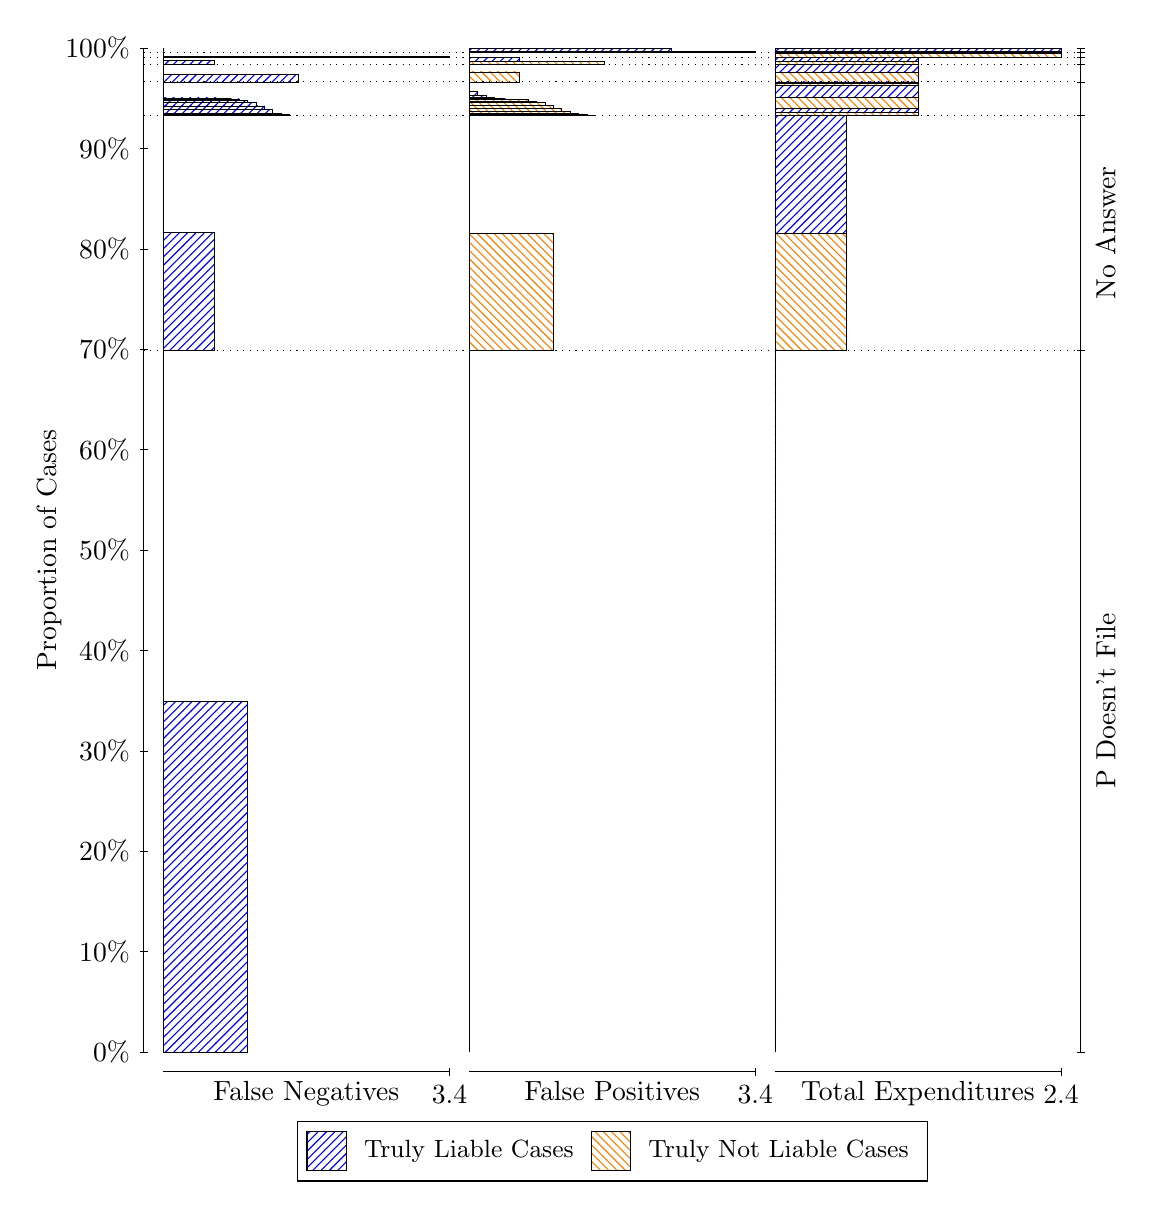
\begin{tikzpicture}
\draw[black, very thin] (1.5,1.75) -- (1.5,14.5);
\node[rotate=90, anchor=center] at (0.3, 8.125) {Proportion of Cases};
\draw[black, very thin] (1.45,1.75) -- (1.55,1.75);
\node[anchor=east] at (1.45, 1.75) {0\%};
\draw[black, very thin] (1.45,3.025) -- (1.55,3.025);
\node[anchor=east] at (1.45, 3.025) {10\%};
\draw[black, very thin] (1.45,4.3) -- (1.55,4.3);
\node[anchor=east] at (1.45, 4.3) {20\%};
\draw[black, very thin] (1.45,5.575) -- (1.55,5.575);
\node[anchor=east] at (1.45, 5.575) {30\%};
\draw[black, very thin] (1.45,6.85) -- (1.55,6.85);
\node[anchor=east] at (1.45, 6.85) {40\%};
\draw[black, very thin] (1.45,8.125) -- (1.55,8.125);
\node[anchor=east] at (1.45, 8.125) {50\%};
\draw[black, very thin] (1.45,9.4) -- (1.55,9.4);
\node[anchor=east] at (1.45, 9.4) {60\%};
\draw[black, very thin] (1.45,10.675) -- (1.55,10.675);
\node[anchor=east] at (1.45, 10.675) {70\%};
\draw[black, very thin] (1.45,11.95) -- (1.55,11.95);
\node[anchor=east] at (1.45, 11.95) {80\%};
\draw[black, very thin] (1.45,13.225) -- (1.55,13.225);
\node[anchor=east] at (1.45, 13.225) {90\%};
\draw[black, very thin] (1.45,14.5) -- (1.55,14.5);
\node[anchor=east] at (1.45, 14.5) {100\%};

\draw[black, very thin] (13.4,1.75) -- (13.4,14.5);
\draw[black, very thin] (13.35,1.75) -- (13.45,1.75);
\node[anchor=west] at (13.35, 1.75) {};
\draw[black, very thin] (13.35,10.663) -- (13.45,10.663);
\node[anchor=west] at (13.35, 10.663) {};
\draw[black, very thin] (13.35,13.643) -- (13.45,13.643);
\node[anchor=west] at (13.35, 13.643) {};
\draw[black, very thin] (13.35,14.071) -- (13.45,14.071);
\node[anchor=west] at (13.35, 14.071) {};
\draw[black, very thin] (13.35,14.292) -- (13.45,14.292);
\node[anchor=west] at (13.35, 14.292) {};
\draw[black, very thin] (13.35,14.379) -- (13.45,14.379);
\node[anchor=west] at (13.35, 14.379) {};
\draw[black, very thin] (13.35,14.448) -- (13.45,14.448);
\node[anchor=west] at (13.35, 14.448) {};
\draw[black, very thin] (13.35,14.5) -- (13.45,14.5);
\node[anchor=west] at (13.35, 14.5) {};

\draw[black, very thin, pattern color=blue, pattern=north east lines] (1.75,1.75) rectangle (2.8186,6.2063);
\draw[black, very thin, pattern color=orange, pattern=north west lines] (1.75,6.2063) rectangle (1.75,10.663);
\draw[black, very thin, pattern color=blue, pattern=north east lines] (1.75,10.663) rectangle (2.3912,12.162);
\draw[black, very thin, pattern color=orange, pattern=north west lines] (1.75,12.162) rectangle (1.75,13.643);
\draw[black, very thin, pattern color=blue, pattern=north east lines] (1.75,13.643) rectangle (3.3529,13.662);
\draw[black, very thin, pattern color=blue, pattern=north east lines] (1.75,13.662) rectangle (3.2461,13.673);
\draw[black, very thin, pattern color=blue, pattern=north east lines] (1.75,13.673) rectangle (3.1392,13.716);
\draw[black, very thin, pattern color=blue, pattern=north east lines] (1.75,13.716) rectangle (3.0324,13.765);
\draw[black, very thin, pattern color=blue, pattern=north east lines] (1.75,13.765) rectangle (2.9255,13.814);
\draw[black, very thin, pattern color=blue, pattern=north east lines] (1.75,13.814) rectangle (2.8186,13.837);
\draw[black, very thin, pattern color=blue, pattern=north east lines] (1.75,13.837) rectangle (2.7118,13.853);
\draw[black, very thin, pattern color=blue, pattern=north east lines] (1.75,13.853) rectangle (2.6049,13.859);
\draw[black, very thin, pattern color=blue, pattern=north east lines] (1.75,13.859) rectangle (2.498,13.866);
\draw[black, very thin, pattern color=orange, pattern=north west lines] (1.75,13.866) rectangle (1.75,14.071);
\draw[black, very thin, pattern color=blue, pattern=north east lines] (1.75,14.071) rectangle (3.4598,14.165);
\draw[black, very thin, pattern color=orange, pattern=north west lines] (1.75,14.165) rectangle (1.75,14.292);
\draw[black, very thin, pattern color=blue, pattern=north east lines] (1.75,14.292) rectangle (2.3912,14.342);
\draw[black, very thin, pattern color=orange, pattern=north west lines] (1.75,14.342) rectangle (1.75,14.379);
\draw[black, very thin, pattern color=blue, pattern=north east lines] (1.75,14.379) rectangle (5.3833,14.39);
\draw[black, very thin, pattern color=orange, pattern=north west lines] (1.75,14.39) rectangle (1.75,14.448);
\draw[black, very thin, pattern color=orange, pattern=north west lines] (1.75,14.448) rectangle (1.75,14.459);
\draw[black, very thin, pattern color=blue, pattern=north east lines] (1.75,14.459) rectangle (1.75,14.5);
\draw[black, very thin, pattern color=orange, pattern=north west lines] (5.6333,1.75) rectangle (5.6333,6.2064);
\draw[black, very thin, pattern color=blue, pattern=north east lines] (5.6333,6.2064) rectangle (5.6333,10.663);
\draw[black, very thin, pattern color=orange, pattern=north west lines] (5.6333,10.663) rectangle (6.702,12.144);
\draw[black, very thin, pattern color=blue, pattern=north east lines] (5.6333,12.144) rectangle (5.6333,13.643);
\draw[black, very thin, pattern color=orange, pattern=north west lines] (5.6333,13.643) rectangle (7.2363,13.649);
\draw[black, very thin, pattern color=orange, pattern=north west lines] (5.6333,13.649) rectangle (7.1294,13.656);
\draw[black, very thin, pattern color=orange, pattern=north west lines] (5.6333,13.656) rectangle (7.0225,13.672);
\draw[black, very thin, pattern color=orange, pattern=north west lines] (5.6333,13.672) rectangle (6.9157,13.697);
\draw[black, very thin, pattern color=orange, pattern=north west lines] (5.6333,13.697) rectangle (6.8088,13.737);
\draw[black, very thin, pattern color=orange, pattern=north west lines] (5.6333,13.737) rectangle (6.702,13.775);
\draw[black, very thin, pattern color=orange, pattern=north west lines] (5.6333,13.775) rectangle (6.5951,13.812);
\draw[black, very thin, pattern color=orange, pattern=north west lines] (5.6333,13.812) rectangle (6.4882,13.821);
\draw[black, very thin, pattern color=orange, pattern=north west lines] (5.6333,13.821) rectangle (6.3814,13.849);
\draw[black, very thin, pattern color=blue, pattern=north east lines] (5.6333,13.849) rectangle (6.1676,13.855);
\draw[black, very thin, pattern color=blue, pattern=north east lines] (5.6333,13.855) rectangle (6.0608,13.861);
\draw[black, very thin, pattern color=blue, pattern=north east lines] (5.6333,13.861) rectangle (5.9539,13.877);
\draw[black, very thin, pattern color=blue, pattern=north east lines] (5.6333,13.877) rectangle (5.8471,13.9);
\draw[black, very thin, pattern color=blue, pattern=north east lines] (5.6333,13.9) rectangle (5.7402,13.949);
\draw[black, very thin, pattern color=blue, pattern=north east lines] (5.6333,13.949) rectangle (5.6333,14.071);
\draw[black, very thin, pattern color=orange, pattern=north west lines] (5.6333,14.071) rectangle (6.2745,14.198);
\draw[black, very thin, pattern color=blue, pattern=north east lines] (5.6333,14.198) rectangle (5.6333,14.292);
\draw[black, very thin, pattern color=orange, pattern=north west lines] (5.6333,14.292) rectangle (7.3431,14.328);
\draw[black, very thin, pattern color=blue, pattern=north east lines] (5.6333,14.328) rectangle (6.2745,14.379);
\draw[black, very thin, pattern color=orange, pattern=north west lines] (5.6333,14.379) rectangle (5.6333,14.437);
\draw[black, very thin, pattern color=blue, pattern=north east lines] (5.6333,14.437) rectangle (5.6333,14.448);
\draw[black, very thin, pattern color=orange, pattern=north west lines] (5.6333,14.448) rectangle (9.2667,14.459);
\draw[black, very thin, pattern color=blue, pattern=north east lines] (5.6333,14.459) rectangle (8.198,14.5);
\draw[black, very thin, pattern color=orange, pattern=north west lines] (9.5167,1.75) rectangle (9.5167,6.2064);
\draw[black, very thin, pattern color=blue, pattern=north east lines] (9.5167,6.2064) rectangle (9.5167,10.663);
\draw[black, very thin, pattern color=orange, pattern=north west lines] (9.5167,10.663) rectangle (10.425,12.144);
\draw[black, very thin, pattern color=blue, pattern=north east lines] (9.5167,12.144) rectangle (10.425,13.643);
\draw[black, very thin, pattern color=orange, pattern=north west lines] (9.5167,13.643) rectangle (11.333,13.683);
\draw[black, very thin, pattern color=blue, pattern=north east lines] (9.5167,13.683) rectangle (11.333,13.732);
\draw[black, very thin, pattern color=orange, pattern=north west lines] (9.5167,13.732) rectangle (11.333,13.875);
\draw[black, very thin, pattern color=blue, pattern=north east lines] (9.5167,13.875) rectangle (11.333,14.026);
\draw[black, very thin, pattern color=orange, pattern=north west lines] (9.5167,14.026) rectangle (11.333,14.049);
\draw[black, very thin, pattern color=blue, pattern=north east lines] (9.5167,14.049) rectangle (11.333,14.071);
\draw[black, very thin, pattern color=orange, pattern=north west lines] (9.5167,14.071) rectangle (11.333,14.198);
\draw[black, very thin, pattern color=blue, pattern=north east lines] (9.5167,14.198) rectangle (11.333,14.292);
\draw[black, very thin, pattern color=orange, pattern=north west lines] (9.5167,14.292) rectangle (11.333,14.328);
\draw[black, very thin, pattern color=blue, pattern=north east lines] (9.5167,14.328) rectangle (11.333,14.379);
\draw[black, very thin, pattern color=orange, pattern=north west lines] (9.5167,14.379) rectangle (13.15,14.437);
\draw[black, very thin, pattern color=blue, pattern=north east lines] (9.5167,14.437) rectangle (13.15,14.448);
\draw[black, very thin, pattern color=orange, pattern=north west lines] (9.5167,14.448) rectangle (13.15,14.459);
\draw[black, very thin, pattern color=blue, pattern=north east lines] (9.5167,14.459) rectangle (13.15,14.5);
\draw[black, dotted] (1.5,10.663) -- (13.4,10.663);
\draw[black, dotted] (1.5,13.643) -- (13.4,13.643);
\draw[black, dotted] (1.5,14.071) -- (13.4,14.071);
\draw[black, dotted] (1.5,14.292) -- (13.4,14.292);
\draw[black, dotted] (1.5,14.379) -- (13.4,14.379);
\draw[black, dotted] (1.5,14.448) -- (13.4,14.448);
\draw[black, very thin] (1.75,1.5) -- (5.3833,1.5);
\node[anchor=north] at (3.5667, 1.5) {False Negatives};
\draw[black, very thin] (5.3833,1.45) -- (5.3833,1.55);
\node[anchor=north] at (5.3833, 1.45) {3.4};

\draw[black, very thin] (5.6333,1.5) -- (9.2667,1.5);
\node[anchor=north] at (7.45, 1.5) {False Positives};
\draw[black, very thin] (9.2667,1.45) -- (9.2667,1.55);
\node[anchor=north] at (9.2667, 1.45) {3.4};

\draw[black, very thin] (9.5167,1.5) -- (13.15,1.5);
\node[anchor=north] at (11.333, 1.5) {Total Expenditures};
\draw[black, very thin] (13.15,1.45) -- (13.15,1.55);
\node[anchor=north] at (13.15, 1.45) {2.4};

\node[black, centered, rotate=90] at (13.72, 6.2063) {P Doesn't File};
\node[black, centered, rotate=90] at (13.72, 12.153) {No Answer};






\draw (7.449999999999999,1.5) node[draw=none] (baseCoordinate) {};
\begin{scope}[align=center]
        \matrix[scale=0.5, draw=black, below=0.5cm of baseCoordinate, nodes={draw}, column sep=0.1cm]{
            \node[rectangle, draw, minimum width=0.5cm, minimum height=0.5cm, pattern=north east lines, pattern color=blue] {}; &
            \node[draw=none, font=\small] (B) {Truly Liable Cases}; &
            \node[rectangle, draw, minimum width=0.5cm, minimum height=0.5cm, pattern=north west lines, pattern color=orange] {}; &
            \node[draw=none, font=\small] (B) {Truly Not Liable Cases}; \\
            };
\end{scope}

\end{tikzpicture}
\end{document}